\subsection{Health and Safety}\label{subsec:healthnsafety}

Since we are working on a pure software project,
we do not interact with any dangerous tools or hardware.
The most fearsome tools for us are actually our office peripherals.
We need to be conscious of the ergonomics of our work environment.


% TODO: add ref, https://www.ccohs.ca/oshanswers/ergonomics/office/monitor_positioning.html
Monitor placement is important because it affects eye strain, and postural strain (neck and shoulders).
It is recommended to keep the monitor approximately forty to seventy cm away from the eyes.
For a quick reference, this is roughly an arm's length away, but it depends on the person.
The monitor height is important as well.
In general, research has found that eyes naturally have a downward cast. % REF.
In fact, they strain more looking above, than looking down.
In practice, guidelines recommend keeping the top of the monitor at eye level, or slightly below.
In general, these are just guidelines to get a good starting point.
It may be worth experimenting depending on the individual's body and what feels best.
A visual summary of these recommendations is given by the Canadian Centre for Occupational Health and Safety (CCOHS) in Figure~\ref{fig:monitor-pos}. % TODO Ref here
\begin{figure}[h]
    \centering
    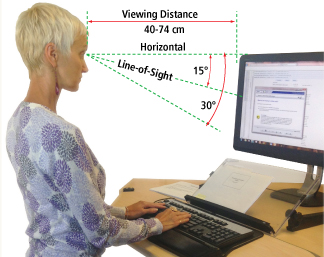
\includegraphics[width=0.5\textwidth]{monitorposition1}
    \caption{The recommended monitor position guidelines from CCOHS.}
    \label{fig:monitor-pos}
\end{figure}

When working for excessively long periods of time without breaks,
it is possible to get repetitive strain injuries (RSI).
It can be from clicking the mouse too much or typing a lot on the keyboard.
Certain mice and keyboards are more ergonomic and help reduce these strains.
They usually have aggressive curves forcing your body to adopt more ergonomic poses.
Office chairs are also an important part of ergonomics, providing proper support while sitting at a desk.

However, even with the best ergonomics setups, the most important is to take frequent breaks from the computer.
Getting up, then walking is good to reduce eye strain, as well as reducing the chances of getting an RSI.
To do this reliably, it is best to set timers and respect them.
Otherwise, there is a risk of getting too absorbed in the work.
After 8 hours of work without breaks writing a report, hands start aching and your body will be the one demanding a break.

% subsection  (end)

\subsection{Engineering Professionalism}\label{subsec:engineering-professionalism}
In ECOR4995, we learned that safety was paramount.

Our first step in addressing this was to analyze the security concerns of our tool.
We do not believe there to be any security vulnerabilities.
This is because it is completely local to the machine, with no internet connection.
We do not believe someone using our tool can harm someone other than themselves by intentionally misusing it.
The only concern would be if an individual delivers falsifies the outputs to provide to someone else.
However, we provide no guarantee for this.
We create text files that can be spoofed without our tool even existing, we decided this concern to be out of scope.

The next question is are there safety concerns, were users can cause harm unintentionally?
We believe there is a way to do so, if our outputs provide false information to a designer.
If the analyzed system is safety critical this can become a safety concern.
The analysis done with our faulty outputs would then compromise the analysis of the safety critical system.
To guard against this, accuracy of our outputs became a critical requirement in our user requirements (see section~\ref{subsubsec:user-reqs}).
We even have a second requirement preferring failure over false positive outputs.

We also made sure to properly licence our program, since we learned that intellectual property was pretty important.

\subsection{Project Management}\label{subsec:project-management}
We started the project by defining some processes for baseline communication and work hours.
That strategy did not work well because we still faced long periods of time without any work or communication.
We had weekly meetings at first, but we wasted time because we had multiple weeks with no work.

The crux of our recovery from this disastrous start came from a pivot towards asynchronous project management with \textbf{GitHub Issues}.
We will look at their purpose in more detail in section~\ref{subsubsec:proj-mngmnt}.
In summary, they were used to formulate task units at a lower level than our requirements.
We could also self-assign the tasks we wanted to do to show to everyone we started work on it.
This is to have a person to contact for status updates, or permission to collaborate on it and avoid duplicating work.

In practice, we stopped doing the assignments because only one person was working for a long period of time.
During the last week before the fair, the team became slightly more active.
Project Management went back to synchronous meetings with dedicated task assignments,
and frequent check-ups to ensure no one was blocked for too long.

We also defined timelines, but they were not respected either.
They only served as a reminder that we were permanently behind schedule, even when we revised our timeline later.
When we switched to Issues, we ended up somewhat ignoring timelines.
We were already working as much as possible until we got blocked, typically due to some lack of understanding of C2KA\@.

Having said that, we still had a clear roadmap of features to follow, and a target date for a first prototype (the fair).
When we were planning tasks, we asked ourselves the feasibility of completion.
This was done in an adhoc manner, based on our knowledge of the current system, and the work left to do.
As we went, we also made sure to mark out of scope features whenever possible (with a rationale) to increase feasibility.
